\documentclass[border=6pt]{standalone}
\usepackage{tikz}
\usetikzlibrary{arrows.meta,positioning,calc,shapes.geometric,fit,backgrounds,patterns,matrix,decorations.pathreplacing}
\begin{document}
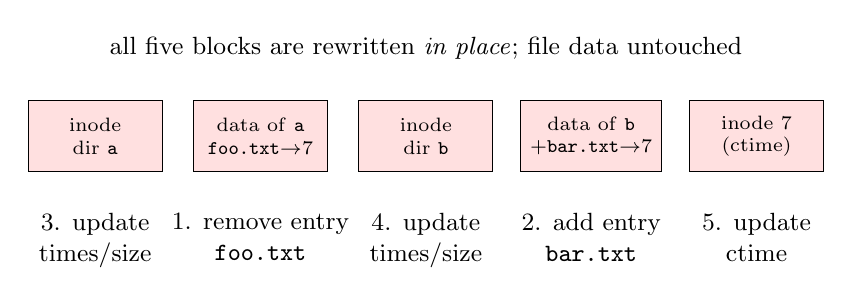
\begin{tikzpicture}[>=Stealth,font=\small]
\tikzstyle{blk}=[draw,minimum width=1.7cm,minimum height=0.9cm,align=center,font=\scriptsize,fill=red!12]
\node[blk] (ia) at (0,0) {inode\\ dir \texttt{a}};
\node[blk] (da) at (2.1,0) {data of \texttt{a}\\ \texttt{foo.txt}$\to$7};
\node[blk] (ib) at (4.2,0) {inode\\ dir \texttt{b}};
\node[blk] (db) at (6.3,0) {data of \texttt{b}\\ +\texttt{bar.txt}$\to$7};
\node[blk] (i7) at (8.4,0) {inode 7\\ (ctime)};
\node[below=0.4cm of da,font=\small,align=center] {1. remove entry\\ \texttt{foo.txt}};
\node[below=0.4cm of db,font=\small,align=center] {2. add entry\\ \texttt{bar.txt}};
\node[below=0.4cm of ib,font=\small,align=center] {4. update\\ times/size};
\node[below=0.4cm of i7,font=\small,align=center] {5. update\\ ctime};
\node[below=0.4cm of ia,font=\small,align=center] {3. update\\ times/size};
\node[above=0.4cm of ib,font=\small] {all five blocks are rewritten \emph{in place}; file data untouched};
\end{tikzpicture}
\end{document}
